\section{Method: TissuePMHC Model for Human Data}

\subsection{Model Overview and Separate Predictions for Each Tissue--HLA Combination (Task-specific Prediction)}

Peptide presentation contains sequence patterns at more than one biological level. Some features may recur across many tissues and \plainHLA{} alleles, whereas others may reflect motifs associated with one allele. TissuePMHC represents these sources with one pathway that learns across all tissue--\plainHLA{} combinations and receives additional tissue and allele guidance during training (global auxiliary branch), and a second pathway that learns only from tissue--\plainHLA{} combinations sharing one \plainHLA{} allele (HLA-specific branch). Each pathway produces a separate score for each biological combination (task-specific score); their orderings within that combination (task) are combined with equal weight and averaged across three independently trained models.

Both pathways use a peptide representation that preserves residue position and examines neighboring residues (position-aware peptide encoder), followed by a separate output layer for each observed tissue--\plainHLA{} combination (task-specific prediction head). This structure allows combinations with many examples to support combinations with few examples (data-rich and data-scarce tasks) without forcing all alleles to use an identical peptide representation. Because the final prediction depends on an output layer learned for a particular tissue--\plainHLA{} combination (task-specific head), the model is not designed for tissue--\plainHLA{} combinations absent from training.

\begin{figure}[tbp]
\centering
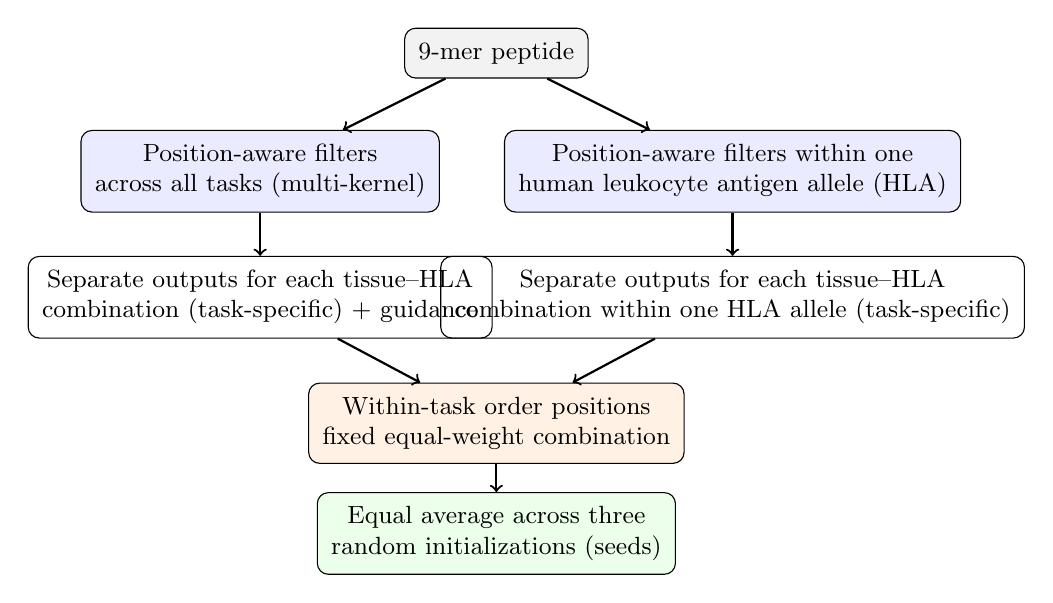
\begin{tikzpicture}[
    box/.style={draw,rounded corners,align=center,inner sep=5pt,font=\small},
    arr/.style={->,thick}
]
\node[box,fill=gray!10] (pep) at (0,0) {9-mer peptide};
\node[box,fill=blue!8] (encg) at (-3,-1.5) {Position-aware filters\\across all tasks (multi-kernel)};
\node[box,fill=blue!8] (ench) at (3,-1.5) {Position-aware filters within one\\human leukocyte antigen allele (HLA)};
\node[box] (global) at (-3,-3.1) {Separate outputs for each tissue--HLA\\combination (task-specific) + guidance};
\node[box] (hla) at (3,-3.1) {Separate outputs for each tissue--HLA\\combination within one HLA allele (task-specific)};
\node[box,fill=orange!10] (fusion) at (0,-4.7) {Within-task order positions\\fixed equal-weight combination};
\node[box,fill=green!8] (seed) at (0,-6.1) {Equal average across three\\random initializations (seeds)};
\draw[arr] (pep) -- (encg);
\draw[arr] (pep) -- (ench);
\draw[arr] (encg) -- (global);
\draw[arr] (ench) -- (hla);
\draw[arr] (global) -- (fusion);
\draw[arr] (hla) -- (fusion);
\draw[arr] (fusion) -- (seed);
\end{tikzpicture}
\caption{Overview of the human model. One pathway learns peptide patterns across all tasks and the other focuses on tissues sharing one \plainHLA{} allele. Predicting tissue and allele labels is used only to guide training (auxiliary objectives); final predictions combine the two within-task orderings and average three independently trained models.}
\label{fig:tissuepmhc-architecture}
\end{figure}

The remainder of this section gives the exact implementation needed for reproduction. Let \(h_i\) denote the numerical representation of peptide \(p_i\), and let \(\tau_i\) be its tissue--\plainHLA{} task. Each pathway (branch) maintains a separate linear output for every available task. The unrestricted score before conversion to a probability (main-task logit) is
\[
z_i=g_{\tau_i}(h_i),
\]
and the associated presentation-preference probability is
\[
q_i=\sigma(z_i),
\]
where \(\sigma\) is the function that converts an unrestricted score to a value between zero and one (logistic sigmoid). During one small training update (a mini-batch update), examples are routed to the separate output layer for their tissue--\plainHLA{} combination (task-specific output layer; task head), while the parameters that create the peptide representation (encoder parameters) are shared according to the pathway definition. The main training penalty is the standard error for a two-class prediction calculated from untransformed output scores (binary cross-entropy with logits; BCE):
\[
\mathcal{L}_{\mathrm{BCE}}
=
-\frac{1}{B}
\sum_{i=1}^{B}
\left[
y_i\log q_i+(1-y_i)\log(1-q_i)
\right].
\]
Although every benchmark pair contains one recorded-positive row and one constructed-negative row (pseudo-negative row), the model processes rows independently and does not use pair identifiers when producing a score (forward pass) or calculating the training penalty (training objective).

\subsection{Peptide Encoding That Preserves Position and Examines Several Motif Lengths}

The biological meaning of an amino acid depends on where it occurs in a 9-mer peptide: anchor positions that stabilize binding to an antigen-presenting molecule (MHC binding) are not interchangeable with other positions. The model component that converts a sequence into numbers (encoder) therefore preserves all nine positions while examining short neighboring patterns of different lengths. For a peptide \(p=(a_1,\ldots,a_9)\), each residue is mapped to a learned vector of 16 numbers (a 16-dimensional embedding), and a learned vector representing its position (positional embedding) is added:
\[
X=E(p)+P \in \mathbb{R}^{9\times d},
\]
where \(E(p)\) contains the learned residue vectors (residue embeddings) and \(P\) is a trainable \(9\times d\) position representation shared across peptides. The learned position vectors (positional embeddings) make the same amino acid distinguishable across locations, which is important because anchor and supporting positions for a \plainMHCI{} molecule are not interchangeable.

The model operates only on standard 9-mer peptides in the present benchmark. No tissue transcriptomics, proteomics, parent-protein sequence, flanking sequence, or external binding score is supplied as input. Tissue and \plainHLA{} information enter through identifiers for tissue--\plainHLA{} combinations (task identities), separate output layers for those combinations (task-specific prediction heads), the rules governing which combinations share model parameters (sharing structure), and additional training-only labels (auxiliary targets), rather than through additional omics measurements.

To examine local sequence patterns spanning two, three, or five residues, we apply sliding one-dimensional filters (one-dimensional convolutions) with widths
\[
\mathcal{K}=\{2,3,5\}.
\]
For each \(k\in\mathcal{K}\), the input is transposed to a channels-first representation and processed as
\[
H_k
=
\operatorname{ReLU}
\left(
\operatorname{Conv1D}_{k}(X)
\right).
\]
Each sliding filter operation (convolution) produces 32 learned feature maps (channels). Boundary values are added temporarily (padding) to retain local context at peptide ends. For even-sized filter windows (kernels), symmetric boundary padding produces one additional position, so the implementation always removes the extra final position (crops the output) to retain nine positions. Consequently, every pathway (branch) yields
\[
H_k\in\mathbb{R}^{9\times 32}.
\]

The three sets of local patterns are joined while preserving their sequence positions. We deliberately avoid reducing the peptide to a position-free maximum or average, because the same short motif can have a different meaning at a different position:
\[
v
=
\operatorname{Flatten}
\left[
H_2;H_3;H_5
\right]
\in\mathbb{R}^{9\cdot32\cdot3}.
\]
The resulting vector is passed through a two-layer feed-forward neural network (\plainMLP{}),
\[
h
=
\operatorname{MLP}(v)
\in\mathbb{R}^{128},
\]
where each intermediate layer (hidden layer) has 128 units and uses a function that keeps positive values and sets negative values to zero (rectified linear unit; ReLU). During training, 20\% of the first layer's activated units are randomly omitted to reduce overfitting (dropout probability 0.2). Joining all position-specific values into one vector (flattening) is deliberate: it allows identical local patterns at different peptide positions to contribute differently to the final representation. The use of \plainMultiKernel{} should be interpreted as a peptide representation tailored to the fixed-length benchmark, rather than as a claim that convolution itself is novel.

\subsection{Information Sharing Across All Tasks and Within One Human Leukocyte Antigen Allele (HLA Allele)}

The pathway that learns across all tasks (global branch) lets every tissue--\plainHLA{} combination contribute to one shared peptide representation. During training, two additional questions guide this representation: does the peptide pattern contain information associated with the recorded tissue, and does it contain information associated with the \plainHLA{} group? These additional training-only predictions (auxiliary objectives) encourage the model to retain biologically relevant grouping information. They do not provide gene expression, protein abundance, or another molecular measurement. Formally, if \(c_i^{(t)}\) and \(c_i^{(m)}\) denote the tissue and \plainHLA{} categories, respectively, the combined training penalty (objective) adds the two-class prediction error described above (BCE) to the standard error for predicting one category among several (categorical cross-entropy; CE):
\[
\mathcal{L}_{\mathrm{global}}
=
\mathcal{L}_{\mathrm{BCE}}
+
\lambda_t
\mathcal{L}_{\mathrm{CE}}
\left(
\widehat{c}^{(t)},c^{(t)}
\right)
+
\lambda_m
\mathcal{L}_{\mathrm{CE}}
\left(
\widehat{c}^{(m)},c^{(m)}
\right),
\]
with fixed weights
\[
\lambda_t=\lambda_m=0.1.
\]
These extra tissue and \plainHLA{} predictions are used only to guide learning and are not consulted when a final peptide score is produced. They should therefore be understood as additional training guidance (auxiliary supervision), not as independent biological evidence.

The second pathway shares information only among tissues with the same \plainHLA{} allele (HLA-specific branch). Its purpose is to preserve allele-associated peptide preferences that broad pooling could blur. For each \plainHLA{} allele \(m\), we define
\[
\mathcal{T}_m
=
\{(t,m)\in\mathcal{T}\}.
\]
A separate sequence-to-vector component (encoder) is trained on the rows belonging to \(\mathcal{T}_m\), and each tissue--\plainHLA{} task in the group receives its own linear output layer (linear head). The training penalty (objective) for allele \(m\) is
\[
\mathcal{L}_{m}
=
\frac{1}{|\mathcal{D}_m|}
\sum_{i\in\mathcal{D}_m}
\mathcal{L}_{\mathrm{BCE}}
\left(
g^{(m)}_{\tau_i}(h_i^{(m)}),y_i
\right).
\]
No additional tissue- or allele-prediction objective (tissue or HLA auxiliary classifier) is used in this pathway. Because every example handled by one allele-restricted model shares the same allele (allele-grouped model), the pathway concentrates its capacity on allele-specific peptide patterns and variation among tissues under the same \plainHLA{} restriction. It complements the pathway shared across all tissue--\plainHLA{} combinations (global branch): broad sharing can stabilize combinations with few examples (long-tailed tasks), whereas sharing restricted to one \plainHLA{} allele can preserve motif structure that unrestricted pooling may blur.

\subsection{Combining the Two Within-task Orderings}

The two pathways are trained separately, so a score of 0.8 from one pathway need not mean the same thing as 0.8 from the other. We therefore compare the ordering produced by each pathway rather than averaging their raw numbers. Within each tissue--\plainHLA{} task, every candidate is converted to its relative position among all candidates (percentile rank). For task \(\tau\), let \(q_{g,i}\) and \(q_{h,i}\) be the two scores for row \(i\):
\[
r_{g,i}
=
\operatorname{PercentileRank}_{\tau}(q_{g,i}),
\qquad
r_{h,i}
=
\operatorname{PercentileRank}_{\tau}(q_{h,i}).
\]
The equal-weight combined prediction (rank-fused prediction) for one \plainSeed{} is
\[
s_i^{(b)}
=
\frac{r_{g,i}+r_{h,i}}{2}.
\]
Both pathways receive fixed equal weight; no tissue or test set is used to choose a preferred pathway. This procedure answers a ranking question, not an absolute probability question. A peptide's percentile depends on the other candidates scored together (evaluation batch), so adding or removing candidates can change its final rank. Prospective use would therefore require either a predefined candidate set or a fixed reference distribution.

\subsection{Averaging Independent Training Runs and Its Scope}

Neural-network training can give slightly different results from different random starting points. We repeat the complete training procedure with three \plainSeeds{} and average the resulting rankings (a multi-seed ensemble) \cite{lakshminarayanan2017deep}:
\[
s_{i,\mathrm{final}}
=
\frac{1}{B}
\sum_{b=1}^{B}
s_i^{(b)},
\qquad B=3.
\]
Thus, the probabilities from each pathway (branch probabilities) are first converted to within-task order positions and combined within each \plainSeed{}; the combined scores are then averaged across \plainSeeds{}. This order is fixed across the \plainFixedTest{}, \plainPairOOF{}, and \plainPeptideOOF{}.

The result from the averaged models (ensemble point estimate) must not be confused with training stability. Averaging three members produces a single prediction vector and therefore cannot by itself demonstrate zero random variation. We separately report the distribution of results from each \plainSeed{}, together with the averaged-model result (ensemble result), so that gains from reducing random training variation remain distinguishable from variation between \plainSeeds{}.

\subsection{Mouse Model That Combines Shared Experts Differently for Each Task}

The mouse analysis tests whether the same biological prediction problem (task) is learnable in a second species; it does not transfer the human model to mouse. We therefore train a separate model that gives equal sampling attention to each tissue--\plainHtwo{} combination during training (task balancing) and combines shared peptide-processing modules differently for each combination (\plainMMoE{}). The model contains three shared peptide-processing modules (experts) and a separate weighting mechanism for each biological combination (task-conditioned gate) that determines their relative contribution for each tissue--\plainHtwo{} context. Each residue has a vector of 16 numbers (16-dimensional representation); the 9-mer is converted to a vector of 128 numbers, processed by three shared modules that each produce 64 numbers (64-dimensional experts), and sent to one of 24 outputs specific to a tissue--\plainHtwo{} combination (task-specific outputs). The model has 68,475 parameters updated during training (trainable parameters).

Because mouse tasks differ in size, every training update draws the same number of rows from each task so that large tissues do not dominate learning (task-balanced sampling). The exact optimization settings are retained for reproducibility: 16 rows are sampled from each of the 24 tasks per update, the model sees the complete training procedure 25 times (25 epochs), its parameters are updated with decoupled weight-decay optimization (AdamW), and models from five \plainSeeds{} are averaged. An additional comparison allows a small adjustment to the peptide representation (an adapter) only for the mouse antigen-presenting-system restriction (H2-Kk); it was chosen before the \plainFixedTest{} was examined.

The TissuePMHC human model and the mouse \plainMMoE{} that was \plainFrozen{} are species-specific methods; no parameter is transferred between them. The comparison tests whether the benchmark question is reproducibly learnable, not whether the models share a representation or biological mechanism.
